\documentclass{article}
\usepackage[utf8]{inputenc}

\title{TPXML - B3231}
\author{Jérôme hue \and Damien Carreau}
\date{February 2020}

\usepackage{natbib}
\usepackage{graphicx}
\usepackage{lmodern}
\usepackage{listings}
\usepackage{geometry}
\geometry{=margin=1cm}

 \usepackage[shortlabels]{enumitem}
                    \setlist[enumerate, 1]{1\textsuperscript{o}}


\begin{document}

\maketitle

\section{Requêtes XPATH}
Dans cette étape, nous devons construire des expressions XPATH pour récupérer des informations sur le document \texttt{countriesTP.xml}.

\begin{enumerate}[1)]

\item Toutes les capitales :\\
    \begin{lstlisting}
    //capital
    \end{lstlisting}
    
    \begin{figure}[h!]
    \centering
    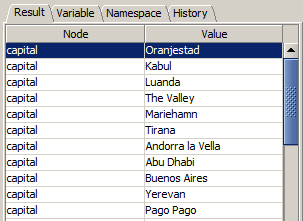
\includegraphics[scale=1]{query1.PNG}
    \caption{Résulat de la requête 1}
    \end{figure}

\item Les noms communs des pays \\
  \begin{lstlisting}
   /countries/country/name/common
    \end{lstlisting}
    
     
    \begin{figure}[h!]
    \centering
    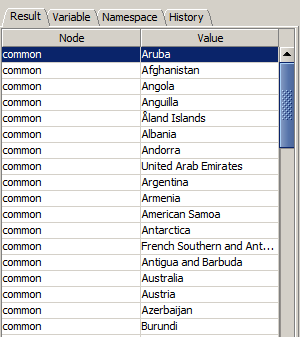
\includegraphics[scale=1]{query2.PNG}
    \caption{Résulat de la requête 2}
    \end{figure}


\item La superficie de chaque pays \\
     \begin{lstlisting}
     //country/@area
    \end{lstlisting}

  
    \begin{figure}[h!]
    \centering
    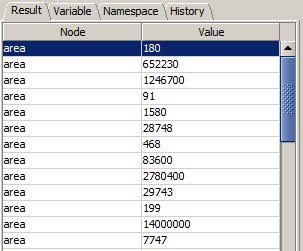
\includegraphics[scale=1]{query3.PNG}
    \caption{Résulat de la requête 3}
    \end{figure}

\newpage
\item Les éléments ayant au moins un attribut \\
    \begin{lstlisting}
    //*[@*]
    \end{lstlisting}
    
   
    \begin{figure}[h!]
    \centering
    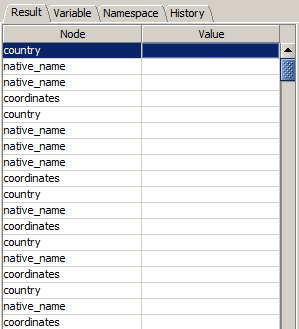
\includegraphics[scale=1]{query4.PNG}
    \caption{Résulat de la requête 4}
    \end{figure}


\item Les Les noms officiels des pays exprimés français, pour ceux qui en ont \\
    \begin{lstlisting}
    //native_name[@lang = 'fra']/official
    \end{lstlisting}

    \begin{figure}[h!]
    \centering
    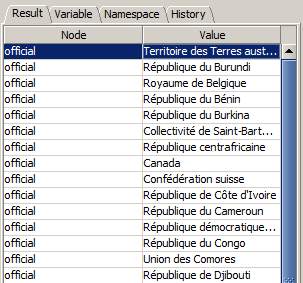
\includegraphics[scale=1]{query5.PNG}
    \caption{Résulat de la requête 5}
    \end{figure}

\item Les Les deuxièmes noms natifs officiels des pays\\
    \begin{lstlisting}
    //name/native_name[position()=2]/official
    \end{lstlisting}
    
   
    \begin{figure}[h!]
    \centering
    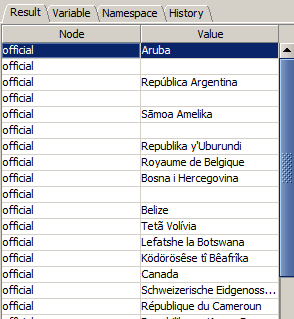
\includegraphics[scale=1]{query6.PNG}
    \caption{Résulat de la requête 6}
    \end{figure}

  

\item La La somme des superficies des pays d'Europe\\
    \begin{lstlisting}
    sum(//country[infosContinent/continent='Europe']/@area)
    \end{lstlisting}

   
    \begin{figure}[h!]
    \centering
    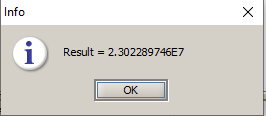
\includegraphics[scale=1]{query7.PNG}
    \caption{Résulat de la requête 7}
    \end{figure}

\item Les Les pays dont le nom commun n'est pas contenu dans leur nom officiel\\
    \begin{lstlisting}
    //name[not(contains(official, common))]/official
    \end{lstlisting}
    
 
    \begin{figure}[h!]
    \centering
    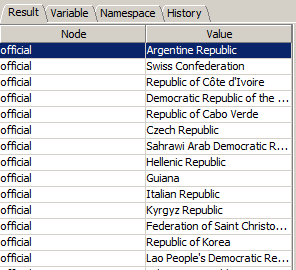
\includegraphics[scale=1]{query8.PNG}
    \caption{Résulat de la requête 8}
    \end{figure}


\item Le dernier voisin de la France\\
    \begin{lstlisting}
    //name[official='French Republic']/../borders/neighbour[last()] \\
    \end{lstlisting}
    
 
    
    Pour avoir le nom complet, on peut effectuer :\\
    \begin{lstlisting}
    //cca3[.=/countries/country/name[official='French Republic']/../
    borders/neighbour[last()]]/../../name/official
    \end{lstlisting}
    
    
    \begin{figure}[h!]
    \centering
    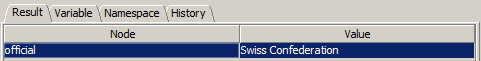
\includegraphics[scale=1]{query9.PNG}
    \caption{Résulat de la requête 9 (deuxième version)}
    \end{figure}
    
    
\item La position de la France dans le document XML \\
    \begin{lstlisting}
    count(//country[name/official = 'French Republic']/preceding-sibling::*)+1
    \end{lstlisting}
    
    \begin{figure}[h!]
    \centering
    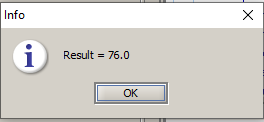
\includegraphics[scale=1]{query10.PNG}
    \caption{Résulat de la requête 10}
    \end{figure}

\item Les langues des noms natifs des pays sans doublons \\
    \begin{lstlisting}
    //native_name[not(preceding::native_name/@lang = @lang)]/@lang
    \end{lstlisting}
    

    \begin{figure}[h!]
    \centering
    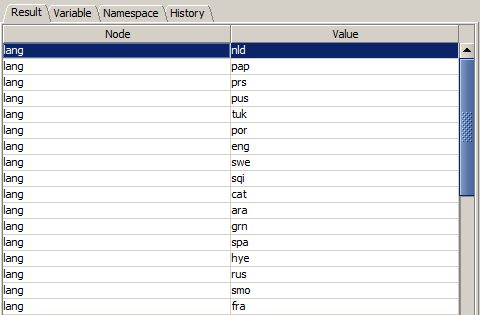
\includegraphics[scale=1]{query11.PNG}
    \caption{Résulat de la requête 11}
    \end{figure}
    
    En XPATH 2.0 :
    \begin{lstlisting}
    distinct-values(//@lang)) 
    \end{lstlisting}
    
    Résultat : on obtient 155 langues.
    
\end{enumerate}




\end{document}
